\documentclass[../main-notes.tex]{subfiles}

\begin{document}

\section{Circle}

A circle is the set of points in a plane that are equidistant from a given point $O$.
The point $O$ is called the center, while the distance $r$ from the center is called the radius.
Twice the radius is known as the diameter $d=2 r$ (fig.\ref{fig:circle}).

\begin{marginfigure}
    \centering
    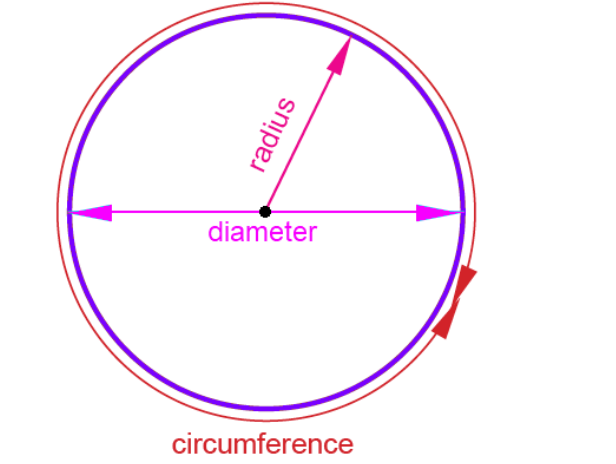
\includegraphics[width=\textwidth]{../Figures/circunference/circle.jpeg}
    \caption{Sketch for the board}\label{fig:circle}
\end{marginfigure}

\subsection{Derivation of the equation}

The main characteristic of the circle is ``\textit{equidistant}'', that is, that the distance between all those points and the point $O$ are equal.
A usefull theorem that translates that characteristic into an equation is the \textbf{Pythagorean theorem}.
Which describes the relationship between the sides of a right triangle (fig.\ref{fig:PitagoreanTheorem}) with the equation,
\begin{gather*}
    a^2 + b^2 = c^2.
\end{gather*}

\begin{marginfigure}
    \centering
    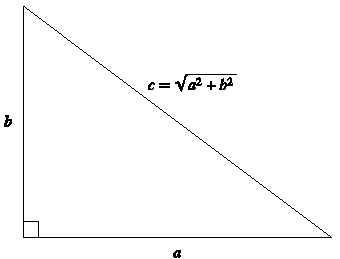
\includegraphics[width=\textwidth]{../Figures/circunference/PythagoreanTheoremFigure_1000.pdf}
    \caption{Sketch for the board for the pythagoream theorem.}\label{fig:PitagoreanTheorem}
\end{marginfigure}

We can show that any point on the circle forms a right triangle with the horizontal and vertical distances from the point $(x,y)$ to the point $O$ (fig.\ref{fig:pit-circle}).
\begin{marginfigure}
    \centering
    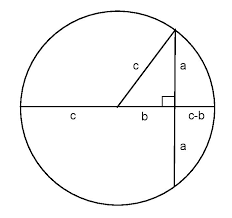
\includegraphics[widht=0.45\textwidth]{../Figures/circunference/pythagoream-circle.png}
    \caption{Relation between pythagorean theorem and the circle.}\label{fig:pit-circle}
\end{marginfigure}
In that sense, we can relate $a$ with $x$, $b$ with $y$ and $c$ with the radius.
In the special case when the radius is equal to one, we have a \textit{unit circle},

\begin{definition}{Unit circle}{~}
    The unit circle is the circle of radius 1 centered at the origin in the $xy$-plane.
    It is represented with the following equation,
    \begin{gather*}
        x^2 + y^2 = 1.
    \end{gather*}
\end{definition}

\subsection{General equation}

Now, let's give the mathematical representation of the point $O$ as $(h,k)$.
Using the knowledge of function translations, we can move the origin of the circle (fig.\ref{fig:circle-translate}) as follows,
\begin{gather}
    \qty(x-h)^2 + \qty(y-k)^2 = r^2.\label{eqn:circle-displaced}
\end{gather}

\begin{marginfigure}
    \centering
    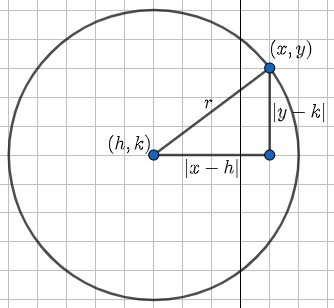
\includegraphics[widht=0.45\textwidth]{../Figures/circunference/circle-translate.jpg}
    \caption{Diplaced circle to the point $(h,k)$.}\label{fig:circle-translate}
\end{marginfigure}

Now, lets get some mathematical exercises.

\begin{note}{Some algebra stuff.}{note-jiji}
    We are going to expand the equation\eqref{eqn:circle-displaced} to get familiarize ourselves with different expressions of the same mathematical object.
    \begin{align*}
        \qty(x-h)^2 + \qty(y-k)^2 &= r^2 \\
        \qty(x^2 -2hx + h^2) + \qty(y^2 -2ky + k^2) &= r^2 \\
        x^2 + y^2 -2hx -2ky + h^2 + k^2 &= r^2
    \end{align*}

    As we can see, this can be approach as a function of two independent variables $x$ and $y$ ($f(x,y)$) equated to a constant value $r^2$, $f(x,y)=r^2$.
    This function is not bijective, indicating that there is no inverse function and the domain and range are bounded.

\end{note}

\subfile{exercise.tex}


Derivation of the equation/function\cref{note:note-jiji}.




Example/Exercises.

\end{document}
